\documentclass[conference]{IEEEtran}
\usepackage[utf8]{inputenc}
\renewcommand{\tablename}{Cuadro}
\renewcommand{\figurename}{Fig.}
\renewcommand{\abstractname}{Resumen}
\usepackage{amsmath,amssymb,amsfonts}
\usepackage{algorithmic}
\usepackage{graphicx}
\usepackage{textcomp}
\usepackage{xcolor}
\usepackage{booktabs}
\usepackage{microtype}
\usepackage{url}
\usepackage{hyperref}

% Configuración de saltos de línea para URLs largas
\def\UrlBreaks{\do\/\do-\do\_}

\hypersetup{
    colorlinks=true,
    linkcolor=blue,
    citecolor=blue,
    urlcolor=blue,
    pdfauthor={Joaquin Basas, Joaquin Alvarado, Johan Quispe},
    pdftitle={Sistema Hibrido Neuro-Simbolico de Vision por Computador y Programacion por Restricciones para la Resolucion de KenKen}
}

\begin{document}

\title{Sistema H\'{\i}brido Neuro-Simb\'olico de Visi\'on por Computador y Programaci\'on por Restricciones para la Resoluci\'on de KenKen}

\author{
    \IEEEauthorblockN{Joaqu\'{\i}n Basas, Joaqu\'{\i}n Alvarado, Johan Quispe}
    \IEEEauthorblockA{\textit{T\'opicos en Ciencias de la Computaci\'on (CC58)} \\
    \textit{Universidad Peruana de Ciencias Aplicadas (UPC)}\\
    Lima, Per\'u \\
    \href{https://github.com/JoanixX/kenken-vision-cp-solver}{\texttt{GitHub: JoanixX/kenken-vision-cp-solver}} \\
    \href{https://huggingface.co/spaces/joako2202/kenken-solver}{\texttt{Demo: joako2202/kenken-solver}}}
}

\maketitle

\begin{abstract}
Este art\'{\i}culo presenta una arquitectura integral neuro-simb\'olica para la extracci\'on, interpretaci\'on y resoluci\'on automatizada de acertijos aritm\'etico-l\'ogicos KenKen a partir de im\'agenes sin procesar. El sistema articula una fase sensorial de visi\'on computacional (rectificaci\'on homogr\'afica $H$, clasificaci\'on de bordes v\'{\i}a Otsu y \textit{Union-Find}, binarizaci\'on adaptativa por desenfoque gaussiano y reconocimiento \'optico de caracteres con una red \texttt{GlyphCNN} adaptada mediante \textit{Fine-Tuning} con \textit{Focal Loss} y miner\'{\i}a de ejemplos dif\'{\i}ciles) con un motor de Programaci\'on por Restricciones (CP) sustentado en Google OR-Tools CP-SAT. Formulamos el problema rigurosamente como un CSP $\langle X, D, C \rangle$, contrastando emp\'{\i}ricamente: (1) modelado aritm\'etico intensional con descomposici\'on de productos y divisi\'on reificada, (2) restricciones globales extensionales de tabla con garant\'{\i}a de Consistencia de Arco Generalizada (GAC), y (3) inferencia conjunta neuro-simb\'olica (MAP) con regularizaci\'on $\ell_0$ para recuperaci\'on robusta ante errores de lectura visual sin incurrir en divergencia. Evaluaciones sistem\'aticas sobre tres corpus (Sint\'etico Normal de 300 im\'agenes, Sint\'etico Dif\'{\i}cil de 150 im\'agenes y un dataset de estr\'es de 50 tableros patol\'ogicos) demuestran una exactitud por glifo del $99.51\%$ y una tasa de resoluci\'on r\'ecord del $90.33\%$ en im\'agenes normales. En an\'alisis de complejidad sobre \'ordenes $n \in [3, 9]$, el solver resuelve tableros de hasta $9 \times 9$ ($1.96 \times 10^{77}$ estados brutos) en menos de $13\text{ ms}$ en el nodo ra\'{\i}z con cero ramas de \textit{backtracking}, logrando una reducci\'on del $39.5\%$ en tiempo de c\'alculo mediante restricciones de tabla en $n=9$. Finalmente, se implementa una pol\'{\i}tica de clasificaci\'on selectiva con opci\'on de rechazo basada en un sem\'aforo de fiabilidad gradual y una interfaz interactiva desplegada en Hugging Face Spaces con 21 muestras operacionales.
\end{abstract}

\begin{IEEEkeywords}
Programaci\'on por Restricciones, KenKen, Inferencia Neuro-Simb\'olica, Restricciones de Tabla, GAC, CP-SAT, Visi\'on por Computador, Focal Loss, Clasificaci\'on Selectiva.
\end{IEEEkeywords}

\section{Introducci\'on}
El acertijo KenKen, creado en 2004 por el pedagogo japon\'es Tetsuya Miyamoto, generaliza la teor\'{\i}a combinatoria de los Cuadrados Latinos al imponer restricciones aritm\'eticas sobre subconjuntos conexos e irregulares de celdas denominados \textit{jaulas} (\textit{cages}). A diferencia de Sudoku, donde la estructura subcuadriculada de $3 \times 3$ es uniforme y r\'{\i}gida, las jaulas de KenKen var\'{\i}an en tama\~no, orientaci\'on espacial y operadores aritm\'eticos ($\{=, +, -, \times, \div\}$). Esto induce un espacio de b\'usqueda combinatorial bruto que escala asint\'oticamente como $\mathcal{O}(n^{n^2})$.

El desaf\'{\i}o cient\'{\i}fico se intensifica cuando el estado del problema no est\'a disponible como una matriz estructurada, sino que debe deducirse a partir de fotograf\'{\i}as f\'{\i}sicas o capturas de pantalla tomadas bajo iluminaci\'on heterog\'enea, sombras proyectadas y distorsi\'on geom\'etrica de perspectiva. En pipelines tradicionales puramente modulares, un \'unico car\'acter o signo mal reconocido por la visi\'on por computador altera las ecuaciones matem\'aticas, transformando una instancia v\'alida en un problema insatisfactible (\texttt{INFEASIBLE}) o conduciendo a soluciones corruptas.

Para solventar esta fragilidad inherente, en este trabajo desarrollamos e implementamos una arquitectura h\'{\i}brida neuro-simb\'olica orientada a la robustez sensorial y eficiencia computacional:
\begin{enumerate}
    \item En la fase sensorial, desacoplamos la geometr\'{\i}a global mediante homograf\'{\i}a proyectiva $H$ y binarizaci\'on adaptativa por desenfoque gaussiano, alimentando una red neuronal convolucional especializada (\texttt{GlyphCNN}) entrenada mediante \textit{Focal Loss} con miner\'{\i}a de ejemplos dif\'{\i}ciles (\textit{Hard Example Mining}) y poda sint\'actica can\'onica por tama\~no de jaula.
    \item En la fase simb\'olica, formulamos el problema formalmente en OR-Tools CP-SAT mediante restricciones globales \texttt{AllDifferent} y restricciones de tabla extensionales que garantizan Consistencia de Arco Generalizada (GAC).
    \item Para la integraci\'on de ambas fases, formulamos un modelo de \textbf{Inferencia Conjunta Neuro-Simb\'olica (Variante C / MAP)} que resuelve simult\'aneamente la coherencia del Cuadrado Latino y la selecci\'on de hip\'otesis visuales veros\'{\i}miles, incorporando una \textbf{penalizaci\'on $\ell_0$ constante} para prevenir mutaciones descontroladas (pseudo-soluciones divergentes).
    \item Implementamos una pol\'{\i}tica de fidedignidad basada en la teor\'{\i}a de clasificaci\'on selectiva y opci\'on de rechazo, proporcionando un sem\'aforo de fiabilidad transparente que audita la fidelidad visual sin censurar soluciones factibles, desplegado en la nube v\'{\i}a Hugging Face Spaces (\url{https://huggingface.co/spaces/joako2202/kenken-solver}).
\end{enumerate}

El c\'odigo fuente del proyecto se encuentra disponible en GitHub (\url{https://github.com/JoanixX/kenken-vision-cp-solver}).

% ==============================================================================
% SECCIÓN II: PIPELINE DE VISIÓN COMPUTACIONAL Y OCR
% ==============================================================================
\section{Pipeline de Visi\'on por Computador y Reconocimiento de Caracteres}
\label{sec:vision_pipeline}

El pipeline sensorial transforma im\'agenes sin procesar en una representaci\'on simb\'olica estructurada. Como se ilustra en la Fig.~\ref{fig:vision_stages}, el procesamiento se divide en: rectificaci\'on geom\'etrica, inferencia topol\'ogica de la grilla, segmentaci\'on morfol\'ogica de glifos y clasificaci\'on probabil\'{\i}stica mediante una red neuronal convolucional adaptada v\'{\i}a \textit{Fine-Tuning}.

\begin{figure*}[t]
\centering
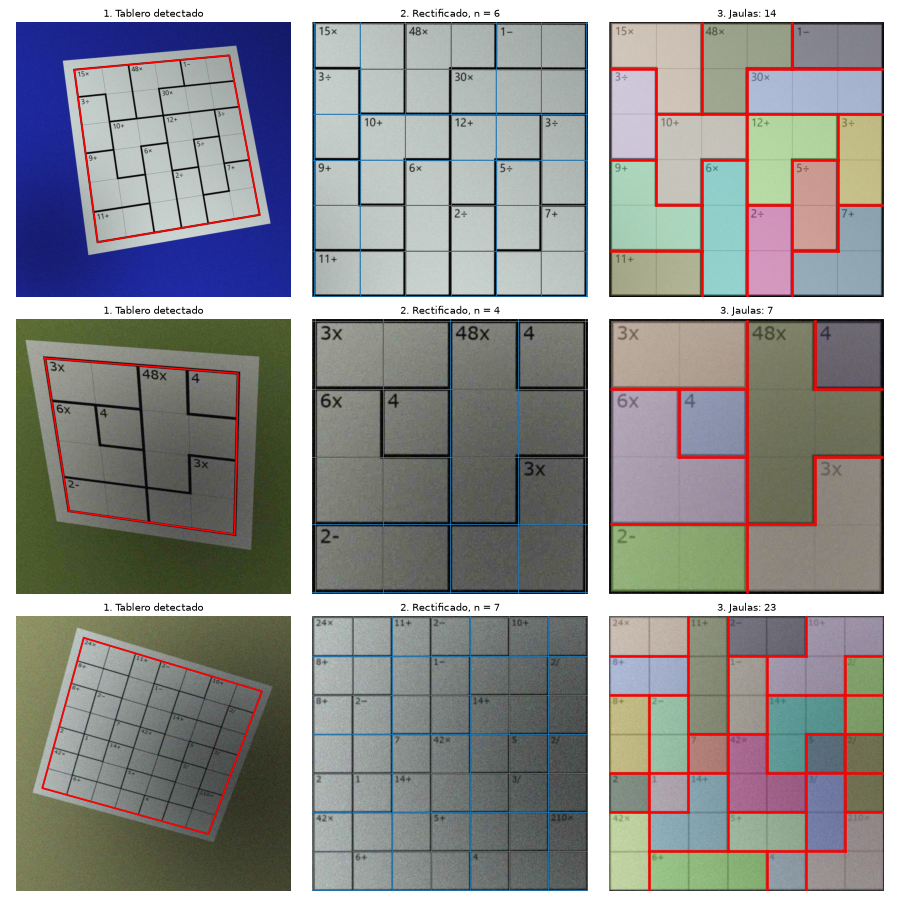
\includegraphics[width=0.95\textwidth]{figs/vision_stages.png}
\caption{Etapas del pipeline de visi\'on computacional: (a) Imagen de entrada con perspectiva y sombras, (b) Binarizaci\'on adaptativa y detecci\'on cuadrangular, (c) Rectificaci\'on proyectiva homogr\'afica $H$, (d) Extracci\'on de l\'{\i}neas y clasificaci\'on de bordes de jaula, (e) Agrupaci\'on conexa por \textit{Union-Find}, y (f) Reconocimiento OCR de etiquetas aritm\'eticas.}
\label{fig:vision_stages}
\end{figure*}

\subsection{Rectificaci\'on Geom\'etrica y Detecci\'on Estructural}
El contorno dominante del tablero se localiza aproximando pol\'{\i}gonos convexos cuadrangulares sobre la imagen binarizada. Para anular la distorsi\'on de perspectiva, se calcula la matriz homogr\'afica proyectiva $H \in \mathbb{R}^{3 \times 3}$~\cite{bradski2000opencv} mapeando las cuatro esquinas hacia un lienzo frontal normalizado de dimensi\'on can\'onica $W \times H$:
\begin{equation}
    \begin{bmatrix} x' \\ y' \\ 1 \end{bmatrix} \sim H \begin{bmatrix} x \\ y \\ 1 \end{bmatrix}
\end{equation}

La inferencia del orden $n \in [3, 9]$ se ejecuta mediante perfiles de proyecci\'on de gradientes morfol\'ogicos verticales y horizontales, identificando la periodicidad espacial de las crestas divisorias.

La separaci\'on entre l\'{\i}neas internas delgadas y bordes gruesos delimitadores de jaula (\textit{cages}) se modela mediante el algoritmo de Otsu~\cite{otsu1979threshold} aplicado sobre los perfiles de intensidad unidimensionales a lo largo de cada frontera entre celdas. Con la matriz de adyacencia de fronteras, se agrupan las celdas conexas pertenecientes a la misma jaula mediante la estructura de datos \textit{Union-Find} con compresi\'on de caminos~\cite{tarjan1975efficiency}, garantizando una complejidad casi lineal $\mathcal{O}(n^2 \alpha(n^2))$.

\subsection{Mejoras Robustas de Preprocesamiento y Segmentaci\'on}
Durante las evaluaciones con degradaci\'on f\'{\i}sica severa, se incorporaron cuatro mecanismos de robustez:
\begin{enumerate}
    \item \textbf{Supresi\'on Perif\'erica de Cuadr\'{\i}cula:} Residuos de las l\'{\i}neas lim\'{\i}trofes de celda distorsionaban el c\'alculo de la altura de referencia tipogr\'afica $h_{\text{ref}}$. La rutina \texttt{clean\_border\_lines} descarta componentes con elongaci\'on vertical ($h \ge 0.35 \cdot h_{\text{celda}}$, $w \le 3\text{ px}$) u horizontal en los bordes marginales ($x \le 2$ o $x \ge w-4$).
    \item \textbf{Binarizaci\'on Adaptativa ante Sombras Locales:} El umbral global de Otsu colapsaba en regiones de iluminaci\'on heterog\'enea cuando la fracci\'on de tinta superaba el 18\%. El sistema conmuta din\'amicamente a una normalizaci\'on de fondo por desenfoque gaussiano de baja frecuencia:
    \begin{equation}
        I_{\text{norm}} = \text{clip}\left(\frac{I}{\mathcal{G}_{\sigma=31}(I)} \times 255, \; 0, \; 255\right)
    \end{equation}
    restituyendo el contraste de glifos en gradientes lum\'{\i}nicos pronunciados.
    \item \textbf{Hip\'otesis Combinadas de Segundo Orden:} En jaulas con n\'umeros de dos d\'{\i}gitos (e.g., $14+$, $48\times$), la proyecci\'on vertical puede fusionar glifos debido al \textit{kerning} estrecho. Se eval\'uan combinaciones m\'ultiples de cortes verticales ponderadas log-probabil\'{\i}sticamente.
    \item \textbf{Poda Sint\'actica Can\'onica a Priori:} Seg\'un las reglas formales de KenKen, los operadores de resta ($-$) y divisi\'on ($\div$) son operaciones binarias no asociativas y est\'an estrictamente restringidas a jaulas de $|V_c| = 2$. Toda hip\'otesis sensorial que asigne $-$ o $\div$ a jaulas de $|V_c| \ge 3$ es podada de forma inmediata, evitando que ruido sensorial introduzca candidatos matem\'aticamente inadmisibles.
\end{enumerate}

\subsection{Clasificador GlyphCNN y Estrategia de Fine-Tuning}
Para el reconocimiento \'optico de caracteres se implement\'o la red convolucional especializada \texttt{GlyphCNN}.

\subsubsection{Arquitectura}
La red procesa recortes normalizados de $32 \times 32$ p\'{\i}xeles en escala de grises. Posee tres bloques convolucionales con normalizaci\'on por lotes (\textit{BatchNorm2D}), activaci\'on ReLU y \textit{MaxPool2D} (filtros 32, 64 y 64), seguidos de \textit{Dropout} ($p=0.25$) y dos capas densas ($512 \to 14$), totalizando $\approx 403{,}000$ par\'ametros entrenables y 14 clases (d\'{\i}gitos $\{0, \dots, 9\}$ y operadores $\{+, -, \times, \div\}$).

\subsubsection{Fine-Tuning con Hard Example Mining y Focal Loss}
Para maximizar la precisi\'on sobre glifos degradados sin alterar la representaci\'on general del modelo base (\texttt{models/ocr\_cnn.pt}, preservado intacto con SHA-256 verificado), se entren\'o una variante especializada (\texttt{models/ocr\_cnn\_finetuned.pt}) mediante:
\begin{itemize}
    \item \textbf{Corpus Focalizado:} 33{,}122 glifos balanceados mediante miner\'{\i}a de ejemplos dif\'{\i}ciles (31{,}093 sint\'eticos con perturbaciones morfol\'ogicas de trazo $x^\gamma$ con $\gamma \in [0.75, 1.35]$, ruido impulsivo y rotaci\'on continua $\pm 10^\circ$; y 2{,}029 glifos recortados de tableros reales degradados).
    \item \textbf{MultiClass Focal Loss:} Formulada con modulaci\'on de clases ambiguas y \textit{Label Smoothing} ($\epsilon = 0.02$)~\cite{lin2017focal}:
    \begin{equation}
        \text{FL}(p_t) = -\alpha_t (1 - p_t)^\gamma \log(p_t)
    \end{equation}
    con $\gamma = 1.5$ y ponderaciones: $\alpha_{\div} = 1.40$, $\alpha_{+} = 1.35$, $\alpha_{-} = 1.25$, $\alpha_{\times} = 1.25$ y $\alpha_{\text{d\'{\i}gitos}} = 1.00$.
    \item \textbf{Congelamiento Selectivo (\textit{Layer Freezing}):} En las \'epocas 1 y 2 se congelaron los filtros de bajo nivel (Bloque 1), adaptando las capas densas con $lr = 2 \times 10^{-4}$. En las \'epocas 3 a 8 se descongel\'o la totalidad de la red con planificador \textit{Cosine Annealing} descendiendo hasta $10^{-5}$.
\end{itemize}

\begin{figure}[htbp]
\centering
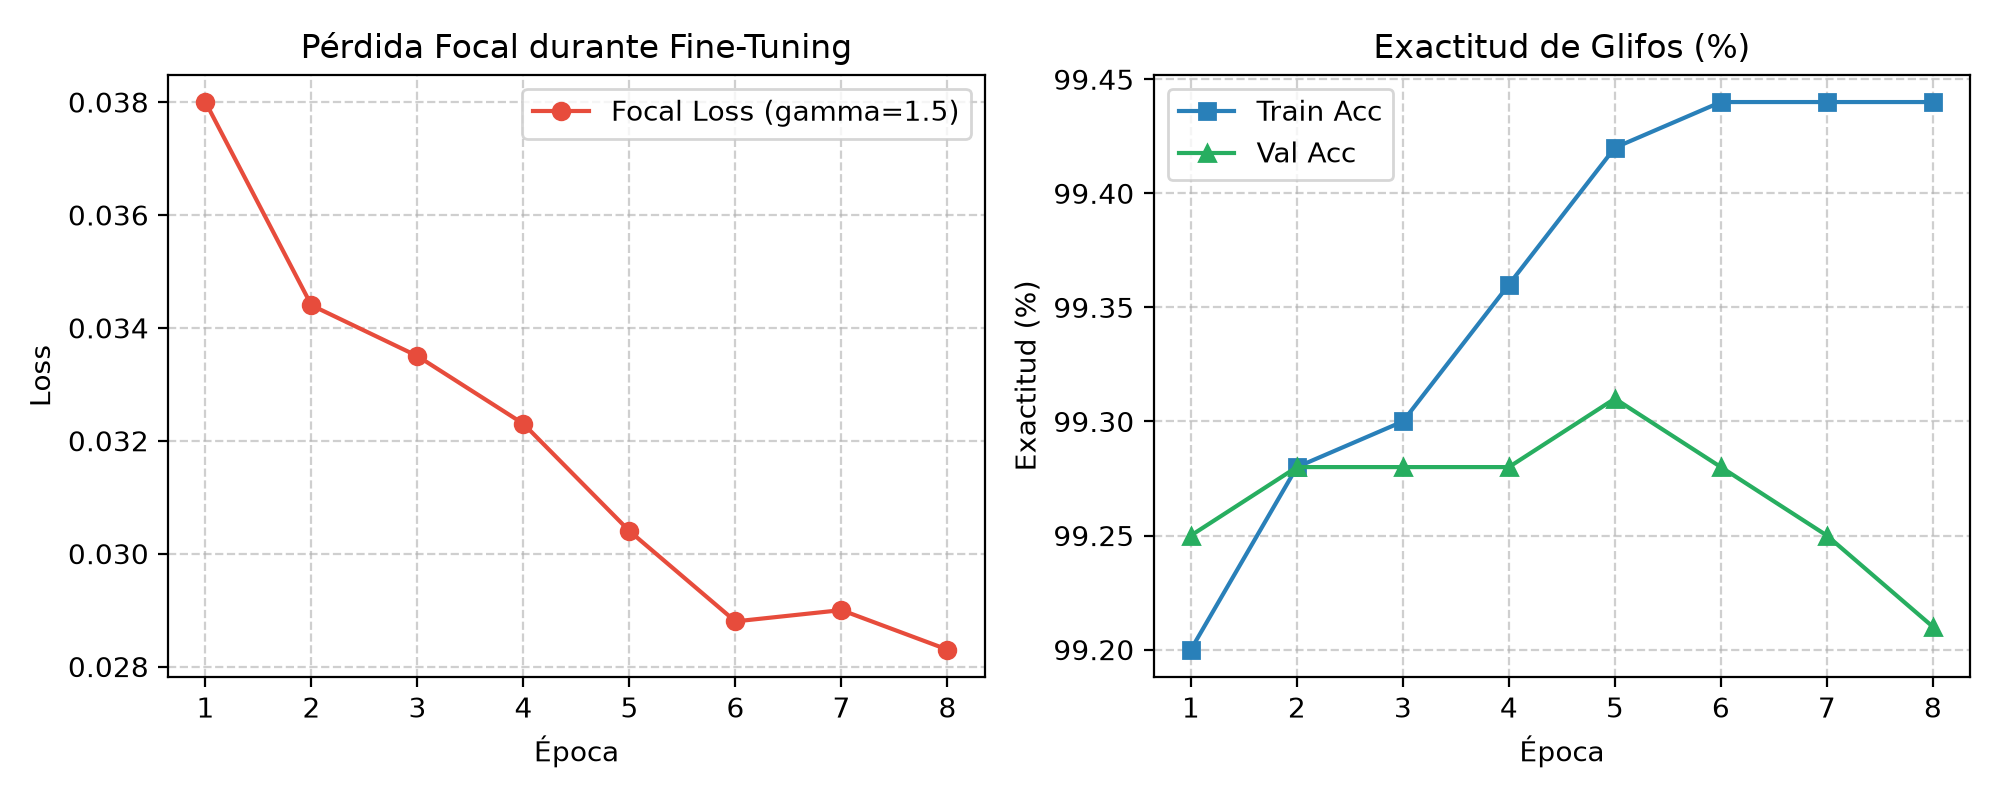
\includegraphics[width=\linewidth]{figs/cnn_finetuning_curves.png}
\caption{Curvas de convergencia del proceso de Fine-Tuning de \texttt{GlyphCNN}: evoluci\'on de la p\'erdida Focal Loss multiclase y exactitud de validaci\'on a lo largo de las 8 \'epocas de entrenamiento.}
\label{fig:cnn_curves}
\end{figure}

Como ilustra la Fig.~\ref{fig:cnn_curves}, el mejor punto de control se consolid\'o en la \'epoca 5 con una exactitud de validaci\'on del $99.31\%$ y p\'erdida de $0.0304$.

\subsection{Evaluaci\'on Experimental y M\'etricas de Error}
El rendimiento del sistema de visi\'on se evalu\'o cuantitativamente en tres entornos:
\begin{enumerate}
    \item \textbf{Synthetic Normal (300 im\'agenes, 12{,}266 glifos):} Tableros bajo iluminaci\'on homog\'enea.
    \item \textbf{Synthetic Hard (150 im\'agenes, 4{,}859 glifos):} Sombras no uniformes, vi\~neteado y ruido de sensor.
    \item \textbf{Challenge Stress (50 im\'agenes, 1{,}778 glifos):} Tableros filtrados donde la lectura Top-1 presenta al menos una inconsistencia o fallo sensorial.
\end{enumerate}

\subsubsection{Comparativa General por Nivel de Entidad}
En el Cuadro~\ref{tab:global_metrics} se contrastan las m\'etricas de reconocimiento por glifo individual, por jaula completa (Top-1 y Top-$k$), y por tablero integral. Mientras que la exactitud por glifo individual en el dataset normal alcanza el $99.51\%$, la exactitud por tablero completo sin asistencia del solver es del $82.00\%$. La integraci\'on de candidatos Top-$k$ junto al motor de CP eleva la tasa de tableros resueltos al récord del \textbf{90.33\%} (271 de 300 tableros).

\begin{table}[htbp]
\caption{M\'etricas de Percepci\'on por Nivel de Entidad y Dataset}
\label{tab:global_metrics}
\centering
\footnotesize
\setlength{\tabcolsep}{3.0pt}
\begin{tabular}{@{}lccc@{}}
\toprule
\textbf{M\'etrica Evaluada} & \textbf{Normal} & \textbf{Hard} & \textbf{Stress} \\
\midrule
Im\'agenes Evaluadas & 300 & 150 & 50 \\
Glifos Analizados & 12{,}266 & 4{,}859 & 1{,}778 \\
Exactitud por Glifo & \textbf{99.51\%} & \textbf{90.99\%} & \textbf{89.43\%} \\
Segmentaci\'on de Jaula OK & 96.50\% & 75.80\% & 80.50\% \\
Jaula Top-1 Exacta & 97.50\% & 74.30\% & 83.80\% \\
Jaula Top-$k$ (con alternativas) & \textbf{99.20\%} & \textbf{84.40\%} & \textbf{93.90\%} \\
Tablero Directo (sin CP) & 82.00\% & 32.00\% & 4.00\% \\
Tablero Resuelto (Top-$k$ + CP) & \textbf{90.33\%} & \textbf{44.67\%} & \textbf{52.00\%} \\
Tiempo Medio por Imagen (s) & 0.261 & 0.365 & 0.387 \\
\bottomrule
\end{tabular}
\end{table}

\subsubsection{Desglose Pormenorizado por Dimensi\'on \texorpdfstring{($n=3$ a $n=9$)}{(n=3 a n=9)}}
El Cuadro~\ref{tab:dim_breakdown} presenta el desglose comparativo exhaustivo por dimensi\'on entre los datasets Synthetic Normal y Synthetic Hard.

\begin{table*}[t]
\caption{Desglose Exhaustivo de M\'etricas de Visi\'on y Resoluci\'on por Dimensi\'on del Tablero \texorpdfstring{($n=3$ a $n=9$)}{(n=3 a n=9)}}
\label{tab:dim_breakdown}
\centering
\footnotesize
\setlength{\tabcolsep}{2.5pt}
\begin{tabular}{@{}cccccccccccc@{}}
\toprule
\textbf{Orden} & \multicolumn{5}{c}{\textbf{Dataset Synthetic Normal (300 tableros)}} & & \multicolumn{5}{c}{\textbf{Dataset Synthetic Hard (150 tableros)}} \\
\cmidrule(lr){2-6} \cmidrule(lr){8-12}
$n$ & \textbf{Cant.} & \textbf{Segm. OK} & \textbf{Jaula Top-1} & \textbf{Tab. Top-1} & \textbf{Tab. + CP} & & \textbf{Cant.} & \textbf{Segm. OK} & \textbf{Jaula Top-1} & \textbf{Tab. Top-1} & \textbf{Tab. + CP} \\
\midrule
$3 \times 3$ & 39 & 98.8\% & 99.4\% & 97.4\% & \textbf{97.4\%} & & 23 & 92.1\% & 95.0\% & 82.6\% & \textbf{91.3\%} \\
$4 \times 4$ & 41 & 98.4\% & 99.7\% & 97.6\% & \textbf{100.0\%} & & 28 & 72.8\% & 77.7\% & 39.3\% & \textbf{50.0\%} \\
$5 \times 5$ & 45 & 98.2\% & 99.4\% & 95.6\% & \textbf{95.6\%} & & 18 & 74.9\% & 75.2\% & 27.8\% & \textbf{27.8\%} \\
$6 \times 6$ & 40 & 97.4\% & 97.7\% & 82.5\% & \textbf{92.5\%} & & 15 & 63.1\% & 60.2\% & 20.0\% & \textbf{33.3\%} \\
$7 \times 7$ & 44 & 97.6\% & 98.7\% & 81.8\% & \textbf{90.9\%} & & 16 & 63.2\% & 59.4\% & 6.2\% & \textbf{12.5\%} \\
$8 \times 8$ & 47 & 96.7\% & 96.7\% & 61.7\% & \textbf{80.9\%} & & 16 & 77.9\% & 77.3\% & 18.8\% & \textbf{43.8\%} \\
$9 \times 9$ & 44 & 94.1\% & 96.3\% & 61.4\% & \textbf{77.3\%} & & 34 & 80.4\% & 77.8\% & 17.6\% & \textbf{38.2\%} \\
\bottomrule
\end{tabular}
\end{table*}

\subsubsection{Comportamiento Falso Positivo y Matriz de Confusi\'on de Glifos}
Las matrices de confusi\'on emp\'{\i}ricas (Fig.~\ref{fig:conf_normal} y Fig.~\ref{fig:conf_hard}) y el desglose de F1-Score por clase (Cuadro~\ref{tab:char_f1}) revelan la naturaleza de los errores sensoriales.

\begin{figure}[htbp]
\centering
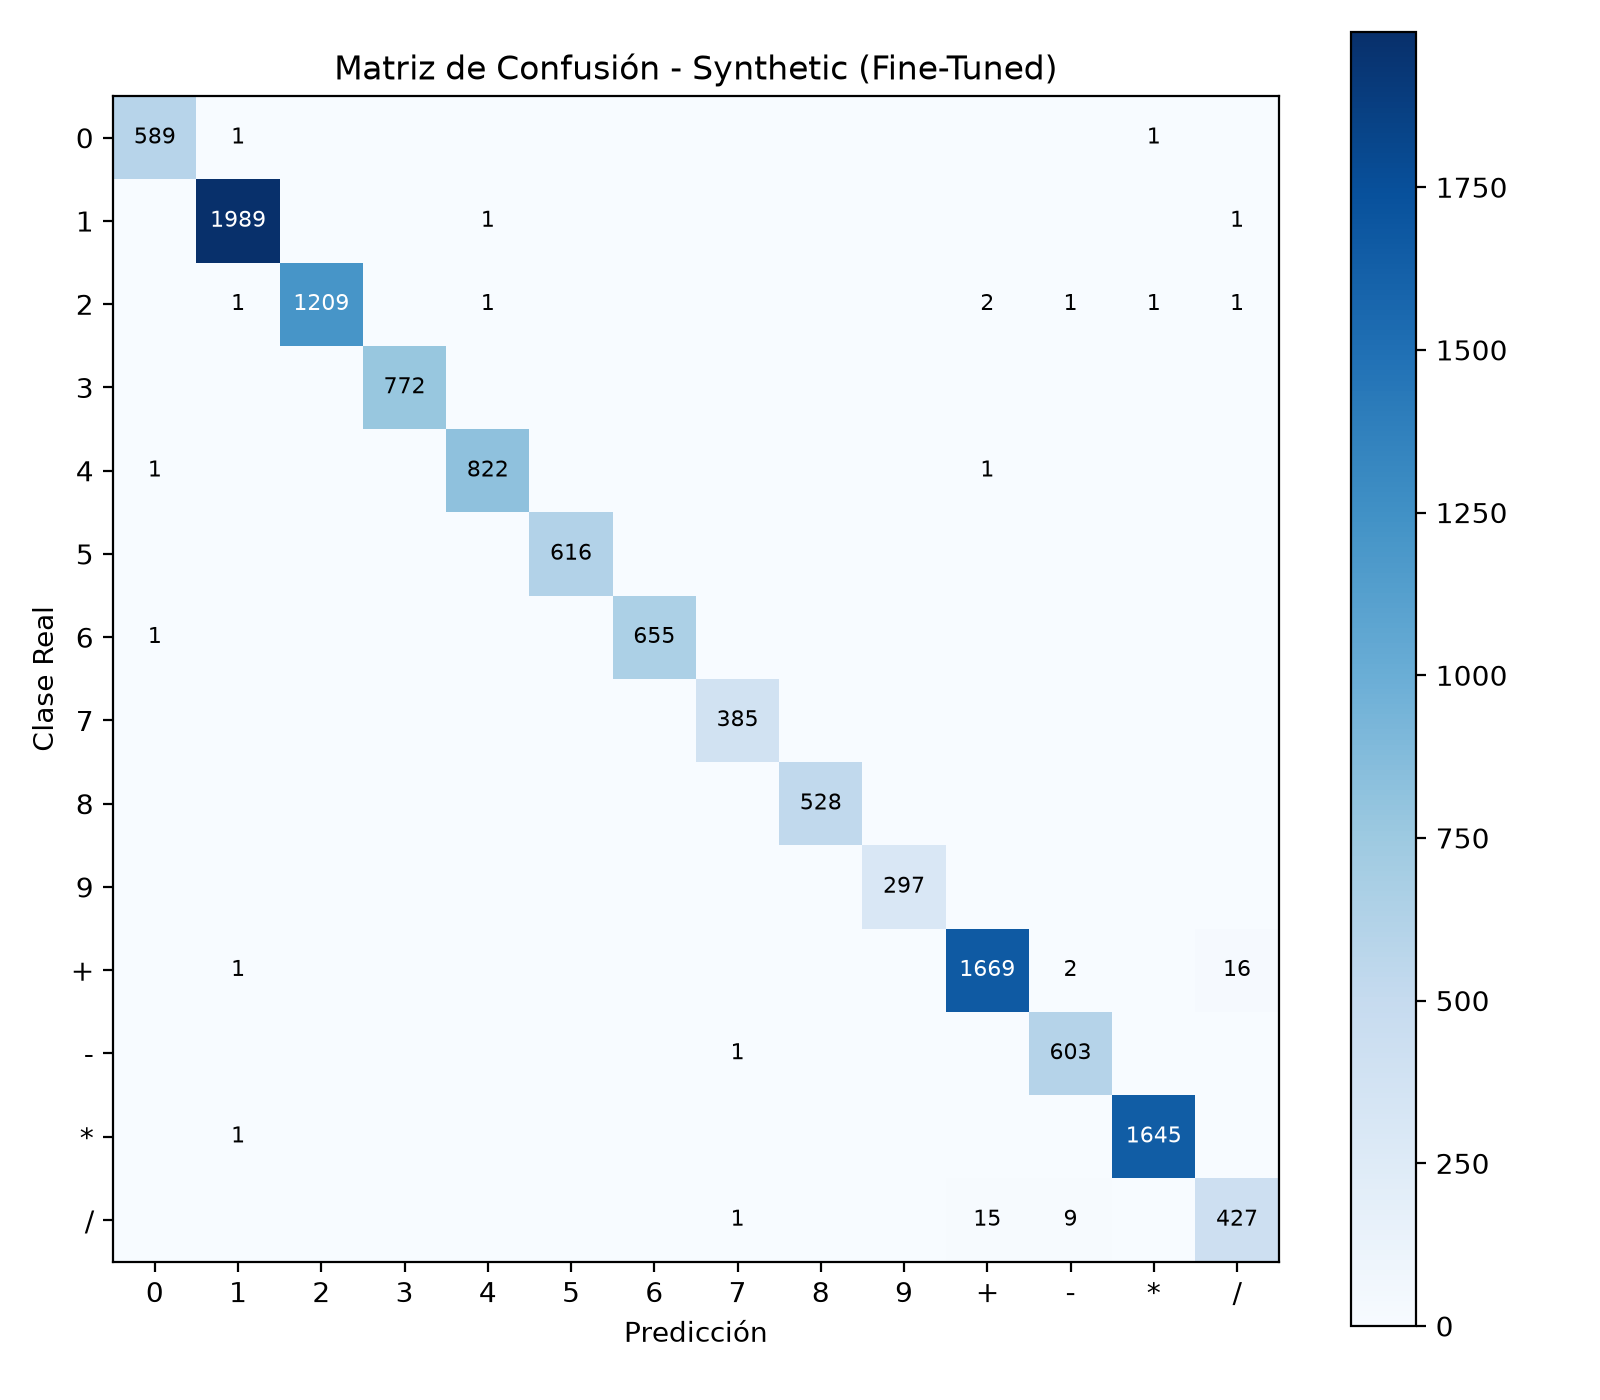
\includegraphics[width=0.88\linewidth]{figs/ocr_finetuned_synthetic_confusion.png}
\caption{Matriz de confusi\'on de \texttt{GlyphCNN} en el dataset Synthetic Normal ($12{,}266$ glifos clasificados).}
\label{fig:conf_normal}
\end{figure}

\begin{figure}[htbp]
\centering
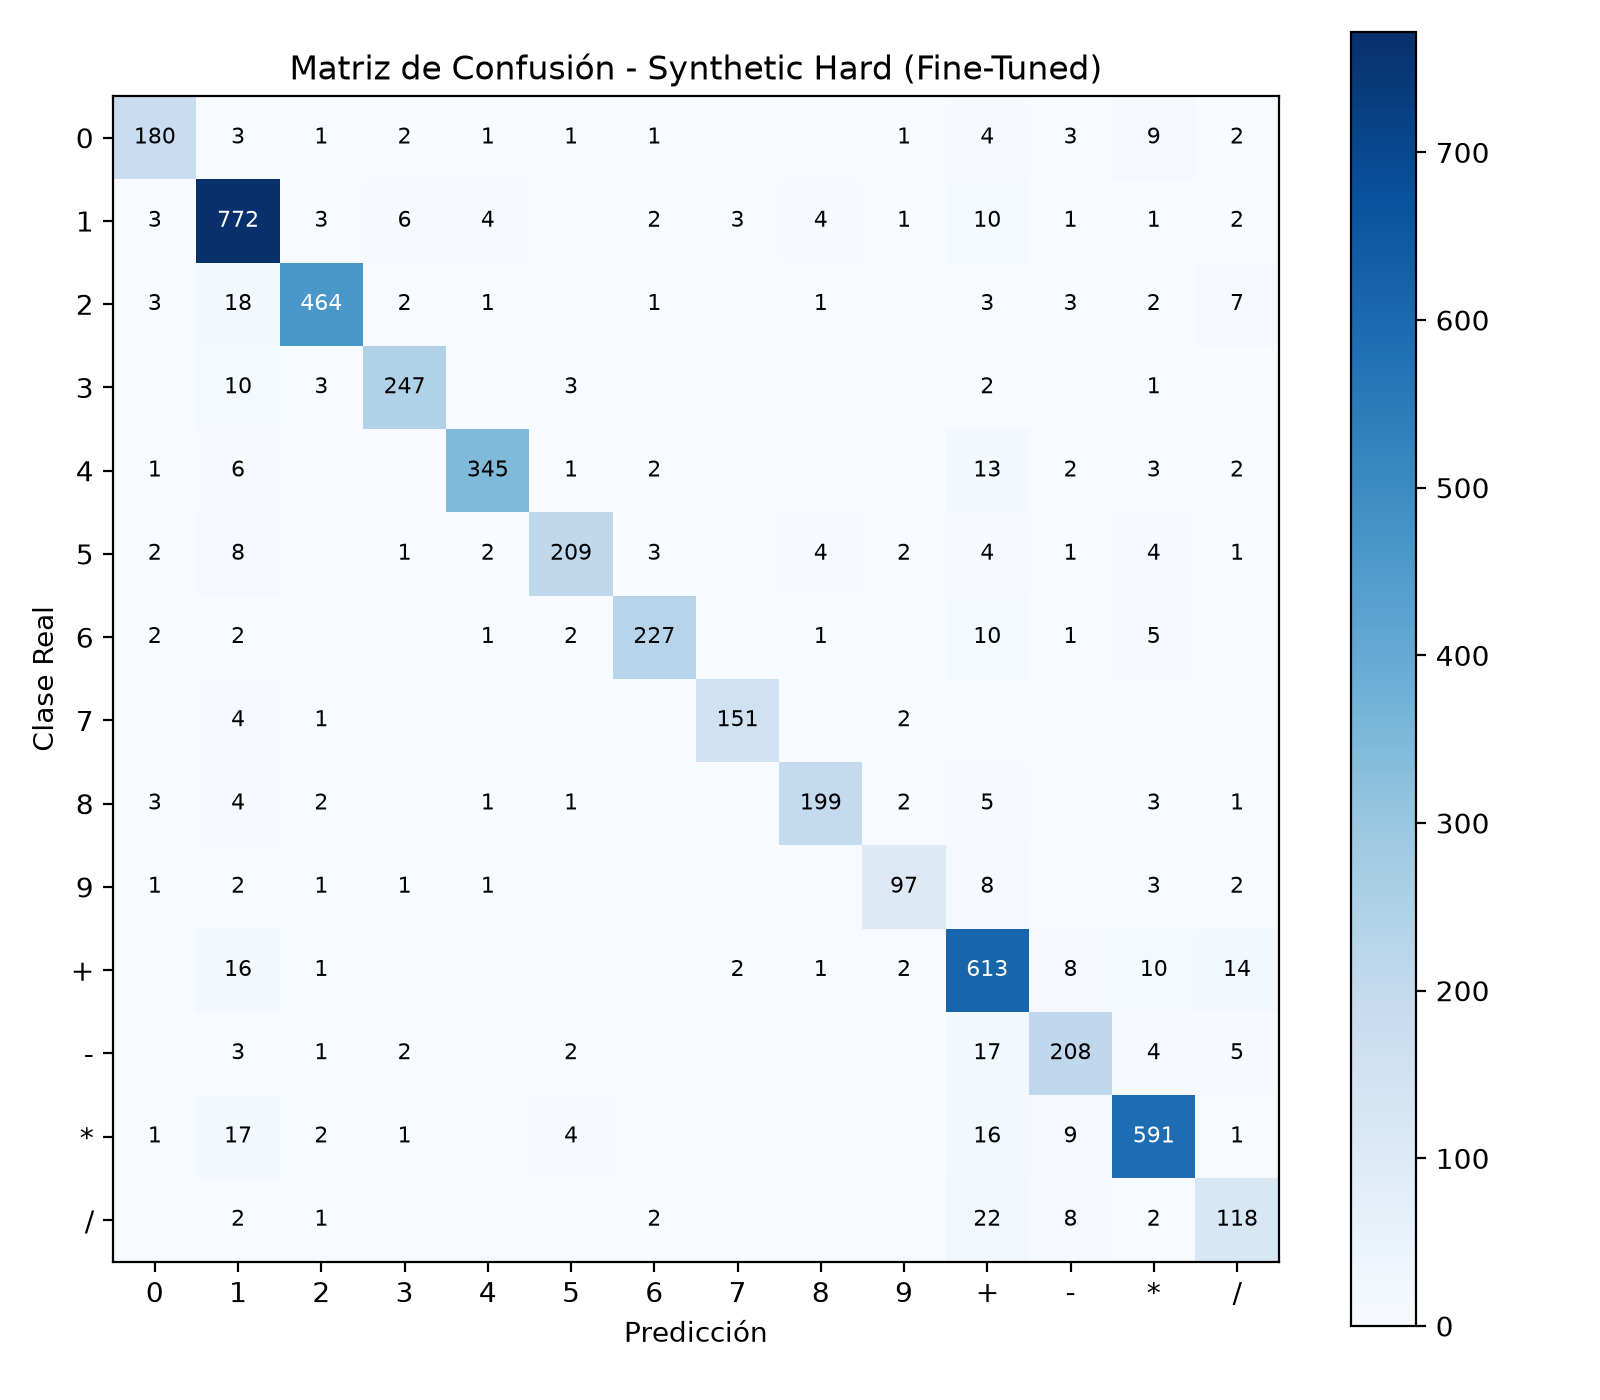
\includegraphics[width=0.88\linewidth]{figs/ocr_finetuned_hard_confusion.png}
\caption{Matriz de confusi\'on de \texttt{GlyphCNN} en el dataset Synthetic Hard ($4{,}859$ glifos con ruido y sombras severas).}
\label{fig:conf_hard}
\end{figure}

\begin{table}[htbp]
\caption{Desempe\~no por Clase: F1-Score (\%) a Trav\'es de los Datasets}
\label{tab:char_f1}
\centering
\footnotesize
\setlength{\tabcolsep}{3.2pt}
\begin{tabular}{@{}ccccc@{}}
\toprule
\textbf{Glifo} & \textbf{F1 Normal} & \textbf{F1 Hard} & \textbf{F1 Stress} & \textbf{Vulnerabilidad} \\
\midrule
$\div$ & 95.21\% & \textbf{76.13\%} & \textbf{70.87\%} & \textbf{Cr\'{\i}tica} \\
$-$    & 98.93\% & 85.60\% & 85.29\% & Alta \\
$+$    & 98.90\% & 87.95\% & 91.24\% & Moderada \\
$\times$& 99.91\% & 92.34\% & 98.55\% & Baja \\
$0$    & 99.66\% & 89.11\% & 94.17\% & Moderada \\
$1$    & 99.85\% & 91.96\% & 95.58\% & Baja \\
$2$    & 99.71\% & 94.21\% & 97.14\% & Baja \\
$3$    & 100.00\% & 93.56\% & 93.72\% & Baja \\
$4$    & 99.76\% & 94.39\% & 98.35\% & Baja \\
$5$    & 100.00\% & 90.09\% & 97.65\% & Moderada \\
$6$    & 99.92\% & 92.84\% & 96.12\% & Baja \\
$7$    & 99.74\% & 96.18\% & 96.70\% & Baja \\
$8$    & 100.00\% & 92.34\% & 98.01\% & Baja \\
$9$    & 100.00\% & 87.00\% & 97.50\% & Moderada \\
\bottomrule
\end{tabular}
\end{table}

Las cinco confusiones f\'{\i}sicas m\'as recurrentes observadas fueron:
\begin{enumerate}
    \item $\div \to +$ (52 casos): La barra oblicua $\div$ al intersectar remanentes de cuadr\'{\i}cula genera un pseudotrazo horizontal que activa los filtros de $+$.
    \item $+ \to \div$ (40 casos): Degradaci\'on lum\'{\i}nica aten\'ua un brazo de $+$, simulando una l\'{\i}nea diagonal ante \'angulos leves de inclinaci\'on.
    \item $- \to +$ (26 casos): Remanentes verticales de la celda que contactan el centro del guion transforman la l\'{\i}nea en cruz.
    \item $2 \to 1$ (24 casos): En celdas de alta densidad ($8\times8$, $9\times9$), los arcos del d\'{\i}gito $2$ pierden contraste, reteniendo \'unicamente el trazo vertical.
    \item $\times \to +$ (18 casos): El glifo de multiplicaci\'on difiere de $+$ \'unicamente por rotaci\'on de $45^\circ$, solapando filtros ante rotaci\'on residual.
\end{enumerate}

% ==============================================================================
% SECCIÓN III: MODELADO CP FORMAL
% ==============================================================================
\section{Modelado Formal mediante Programaci\'on por Restricciones (CP)}
\label{sec:cp_modeling}

El acertijo KenKen de orden $n$ se formaliza como un CSP $\mathcal{P} = \langle X, D, C \rangle$, donde $X$ es el conjunto de variables de decisi\'on, $D$ sus dominios y $C$ el conjunto de restricciones.

\subsection{Variables de Decisi\'on y Dominios}
Para una cuadr\'{\i}cula de $n \times n$, se define:
\begin{equation}
    X = \{x_{i,j} \mid 1 \le i \le n, \; 1 \le j \le n\}
\end{equation}
donde cada variable $x_{i,j}$ denota el d\'{\i}gito en la fila $i$ y columna $j$, con dominio uniforme:
\begin{equation}
    D(x_{i,j}) = \{1, 2, \dots, n\}, \quad \forall x_{i,j} \in X
\end{equation}
El problema contiene $n^2$ variables. La colecci\'on de jaulas $\mathcal{C} = \{c_1, \dots, c_m\}$ conforma una partici\'on exacta del tablero:
\begin{equation}
    \bigcup_{c \in \mathcal{C}} V_c = X \quad \land \quad V_a \cap V_b = \emptyset, \quad \forall a \ne b
\end{equation}
donde cada jaula $c = \langle V_c, T_c, \text{op}_c \rangle$ est\'a definida por sus celdas $V_c \subseteq X$, objetivo num\'erico $T_c \in \mathbb{N}$ y operador $\text{op}_c \in \{=, +, -, \times, \div\}$.

\subsection{Restricciones Globales de Tablero (Cuadrado Latino)}
Se imponen restricciones de desigualdad sobre cada fila y columna mediante el algoritmo de filtrado de R\'egin~\cite{regin1994filtering}:
\begin{align}
    \text{AllDifferent}(\{x_{i,1}, x_{i,2}, \dots, x_{i,n}\}), & \quad \forall i \in \{1, \dots, n\} \label{eq:alldiff_row} \\
    \text{AllDifferent}(\{x_{1,j}, x_{2,j}, \dots, x_{n,j}\}), & \quad \forall j \in \{1, \dots, n\} \label{eq:alldiff_col}
\end{align}

Adicionalmente, se modelan restricciones redundantes de suma triangular de Gauss:
\begin{equation}
    \sum_{j=1}^n x_{i,j} = \frac{n(n+1)}{2}, \quad \sum_{i=1}^n x_{i,j} = \frac{n(n+1)}{2}
    \label{eq:redundant_sum}
\end{equation}

\subsection{Modelado de Jaulas: Variante A (Aritm\'etica Intensional)}
\begin{enumerate}
    \item \textbf{Identidad ($=$):} Para jaulas unarias ($|V_c| = 1$): $v_1 = T_c$.
    \item \textbf{Suma ($+$):} Restricci\'on lineal global: $\sum_{v \in V_c} v = T_c$.
    \item \textbf{Multiplicaci\'on ($\times$):} Descomposici\'on encadenada mediante variables auxiliares enteras $p_k \in [1, n^{k+1}]$ implementada v\'{\i}a \texttt{AddMultiplicationEquality}:
    \begin{equation}
    \begin{aligned}
        p_1 &= v_1 \cdot v_2, \\
        p_k &= p_{k-1} \cdot v_{k+1} \quad (k \ge 2), \\
        T_c &= p_{|V_c|-2} \cdot v_{|V_c|}
    \end{aligned}
    \end{equation}
    \item \textbf{Diferencia Absoluta ($-$):} $|v_1 - v_2| = T_c \iff \text{AddAbsEquality}(T_c, v_1 - v_2)$.
    \item \textbf{Divisi\'on Reificada ($\div$):} Reificaci\'on l\'ogica condicional con variable booleana de direcci\'on $b_{\text{dir}} \in \{0, 1\}$ y \texttt{OnlyEnforceIf}:
    \begin{align}
        b_{\text{dir}} &\implies v_1 = T_c \cdot v_2 \label{eq:div_reif_1} \\
        \neg b_{\text{dir}} &\implies v_2 = T_c \cdot v_1 \label{eq:div_reif_2}
    \end{align}
\end{enumerate}

\subsection{Modelado de Jaulas: Variante B (Restricciones Globales de Tabla)}
Cada jaula se formula de manera extensional mediante el cat\'alogo de asignaciones v\'alidas $\mathcal{T}_c \subset \{1, \dots, n\}^{|V_c|}$ con \texttt{AddAllowedAssignments}:
\begin{equation}
    \text{AllowedAssignments}(V_c, \mathcal{T}_c)
    \label{eq:table_constraint}
\end{equation}
El algoritmo aplica filtrado topol\'ogico a priori: tuplas que repitan valores en celdas alineadas en la misma fila o columna son podadas antes de compilar el modelo, garantizando \textbf{Consistencia de Arco Generalizada (GAC)}~\cite{bessiere2006table} en el nodo ra\'{\i}z.

\subsection{Variante C: Inferencia Conjunta Neuro-Simb\'olica v\'{\i}a Reificaci\'on con Regularizaci\'on \texorpdfstring{$\ell_0$}{L0}}
Para tolerar errores de lectura, se formula un problema de M\'axima Verosimilitud Consistente (MAP)~\cite{deraedt2011constraint}. Con $K_c$ candidatos de lectura y probabilidades normalizadas $P_{c,k}$, se introducen variables indicadoras:
\begin{equation}
    r_{c,k} \in \{0, 1\}, \quad \forall c \in \mathcal{C}, \; \forall k \in \{0, \dots, K_c - 1\}
\end{equation}
sujetas a:
\begin{equation}
    \text{ExactlyOne}(\{r_{c,0}, r_{c,1}, \dots, r_{c,K_c - 1}\}), \quad \forall c \in \mathcal{C}
\end{equation}
\begin{equation}
    r_{c,k} \implies \mathcal{A}(V_c, T_{c,k}, \text{op}_{c,k})
\end{equation}

Para evitar mutaciones descontroladas de jaulas, se incorpora una \textbf{penalizaci\'on $\ell_0$ constante} $\lambda_{\text{change}} = 1.5$ ($1500$ unidades enteras):
\begin{equation}
\begin{aligned}
    \max \sum_{c \in \mathcal{C}} \sum_{k=0}^{K_c - 1} r_{c,k} \cdot \Big( & \lfloor 1000 \cdot \log P_{c,k} \rfloor \\
    & - \mathbf{1}_{\{k > 0\}} \cdot 1500 \Big)
\end{aligned}
\label{eq:map_objective_l0}
\end{equation}
y se audita deterministamente:
\begin{equation}
    M_{\text{corregidas}} = \sum_{c \in \mathcal{C}} \sum_{k=1}^{K_c - 1} r_{c,k}
\end{equation}

% ==============================================================================
% SECCIÓN IV: COMPLEJIDAD Y RESULTADOS DEL SOLVER
% ==============================================================================
\section{An\'alisis de Complejidad y Evaluaci\'on Experimental del Solver}
\label{sec:complexity_and_experiments}

\subsection{Complejidad Te\'orica vs. Espacio de B\'usqueda Podado}
El espacio de b\'usqueda bruto escala seg\'un $|\mathcal{S}_{\text{bruto}}| = n^{n^2} = \mathcal{O}(n^{n^2})$. Para $n=3$, $|\mathcal{S}| = 19{,}683$. Para $n=9$, el espacio combinatorial alcanza $9^{81} \approx 1.96 \times 10^{77}$ estados factibles brutos.

Al imponer la restricci\'on de Cuadrado Latino por filas, el espacio se reduce a $(n!)^n$ ($1.09 \times 10^{50}$ en $n=9$). CP-SAT~\cite{perron2023cpsat, perron2024ortools} integra \textit{Lazy Clause Generation} (LCG)~\cite{ohrimenko2009lazy}, resolviendo las instancias directamente en el \textbf{nodo ra\'{\i}z} con cero ramas de \textit{backtracking}.

\subsection{Resultados Experimentales del Benchmark CP-SAT \texorpdfstring{($n=3$ a $n=9$)}{(n=3 a n=9)}}
Se ejecutaron 12 repeticiones independientes por orden y formulaci\'on desde $n=3$ hasta $n=9$. Los resultados promedio de tiempo (\textit{Wall Time}), ramas y conflictos se detallan en el Cuadro~\ref{tab:cp_benchmark} y la Fig.~\ref{fig:cp_benchmark}.

\begin{table}[!htbp]
\caption{Comparativa Experimental de Rendimiento del Solver CP-SAT \texorpdfstring{($n=3$ a $n=9$)}{(n=3 a n=9)}}
\label{tab:cp_benchmark}
\centering
\footnotesize
\setlength{\tabcolsep}{2.0pt}
\noindent\resizebox{\columnwidth}{!}{%
\begin{tabular}{@{}ccccccc@{}}
\toprule
\textbf{Orden} & \textbf{Espacio Bruto} & \multicolumn{4}{c}{\textbf{Wall Time Medio (ms)}} & \textbf{Ramas} \\
\cmidrule(lr){3-6}
$n$ & $n^{n^2}$ & \textbf{Var. A} & \textbf{A+Red} & \textbf{Var. B} & \textbf{B+Red} & \textbf{Medias} \\
\midrule
3 & $1.97 \times 10^4$  & 9.07  & 15.26 & 15.00 & 14.47 & \textbf{0} \\
4 & $4.29 \times 10^9$  & 10.38 & 14.28 & 15.46 & 14.70 & \textbf{0} \\
5 & $2.98 \times 10^{17}$ & 13.53 & 14.56 & 14.51 & 14.46 & \textbf{0} \\
6 & $1.03 \times 10^{28}$ & 9.54  & 14.39 & 15.42 & 14.22 & \textbf{0} \\
7 & $2.56 \times 10^{41}$ & 9.23  & 14.56 & 13.68 & 14.26 & \textbf{0} \\
8 & $6.28 \times 10^{57}$ & 12.68 & 14.31 & 13.25 & 12.18 & \textbf{0} \\
9 & $1.96 \times 10^{77}$ & 20.03 & 13.03 & \textbf{12.11} & 17.22 & \textbf{0} \\
\bottomrule
\end{tabular}%
}
\end{table}

\begin{figure}[!htbp]
\centering
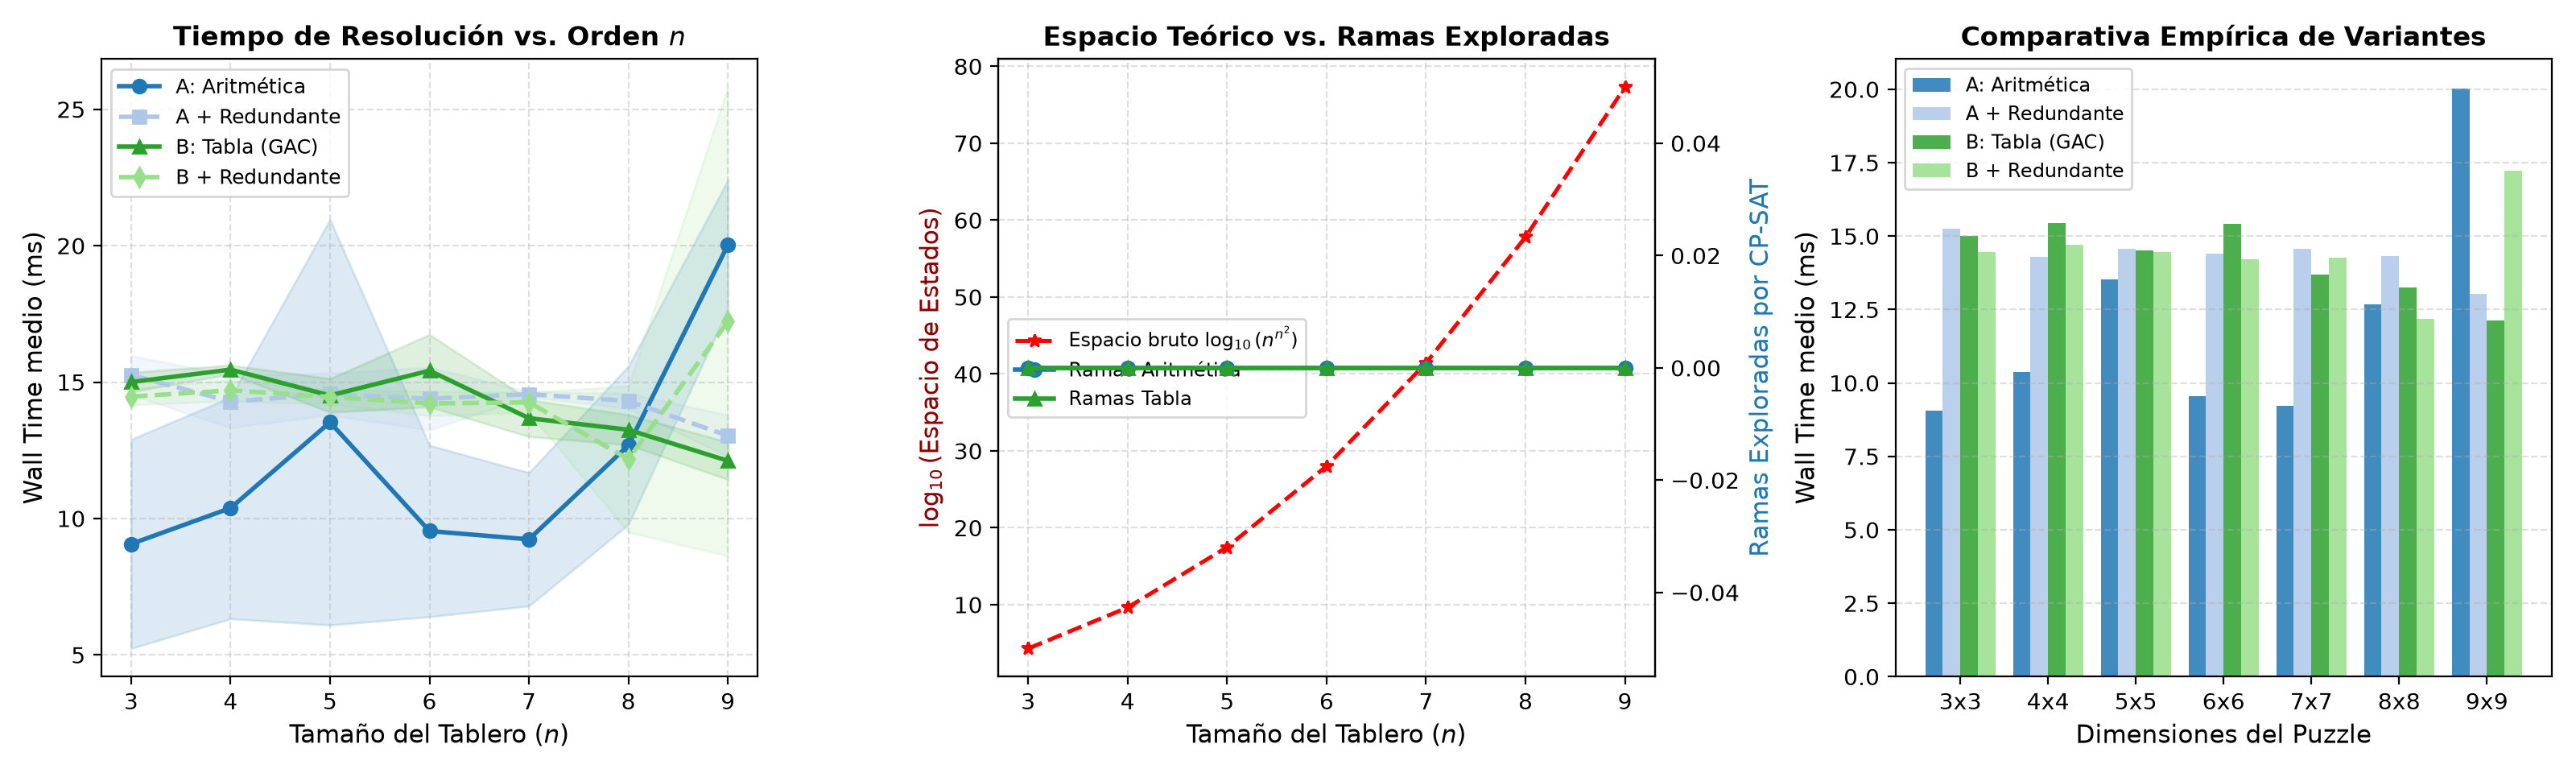
\includegraphics[width=\linewidth]{figs/cp_benchmark.png}
\caption{Evaluaci\'on emp\'{\i}rica del solver CP-SAT ($n=3$ a $9$): (a) Tiempo de ejecuci\'on medio por variante de modelado, (b) Crecimiento exponencial del espacio de estados bruto en escala logar\'{\i}tmica, (c) Ramas exploradas y conflictos reportados por el solver.}
\label{fig:cp_benchmark}
\end{figure}

\subsection{Discusi\'on de Hallazgos Emp\'{\i}ricos}
\begin{enumerate}
    \item \textbf{Aceleraci\'on GAC en Gran Escala (Variante B):} En $n=9$, la Variante B extensional resolvi\'o en \textbf{12.11 ms} frente a 20.03 ms de la Variante A intensional (reducci\'on neta del \textbf{39.5\%}). El filtrado GAC de tabla poda valores inconsistentes antes de iniciar la propagaci\'on booleana.
    \item \textbf{Efecto de Restricciones Redundantes:} Para $n=9$, la suma Gaussiana aceler\'o la formulaci\'on intensional en un $35\%$ ($20.03\text{ ms} \to 13.03\text{ ms}$).
    \item \textbf{Resoluci\'on en Nodo Ra\'{\i}z con Cero Backtracking:} En todas las dimensiones evaluadas se observaron exactamente \textbf{0 ramas} y \textbf{0 conflictos}.
\end{enumerate}

% ==============================================================================
% SECCIÓN V: FIDEDIGNIDAD Y ABSTENCIÓN HONESTA
% ==============================================================================
\section{Pol\'{\i}tica de Fidedignidad, Mitigaci\'on de Divergencia y Sem\'aforo de Fiabilidad}
\label{sec:reliability}

\subsection{El Dilema \'Etico-T\'ecnico: Falso \'Exito vs. Abstenci\'on Honesta}
En sistemas neuro-simb\'olicos, si la etiqueta verdadera de una jaula no figura en el Top-$k$ de la CNN, un solver CP sin regularizar puede permutar m\'ultiples jaulas hacia opciones inveros\'{\i}miles para forzar la satisfactibilidad del Cuadrado Latino. El sistema reporta \texttt{OPTIMAL}, pero entregando una soluci\'on para un \textbf{tablero diferente al impreso en papel}. Este fen\'omeno de \textbf{Divergencia (Pseudo-soluci\'on)} ocurri\'o en el $32.0\%$ del dataset de estr\'es.

\subsection{Marco Te\'orico: Clasificaci\'on Selectiva y Opci\'on de Rechazo}
Siguiendo la teor\'{\i}a de \textit{Reject Option} de Chow~\cite{chow1970optimum} y Cortes et al.~\cite{cortes2016learning}, el coste del error no detectado ($c_{\text{error}}$, entregar un tablero falso) es significativamente superior al coste de la abstenci\'on honesta ($c_{\text{abstain}}$, advertir degradaci\'on de la imagen).

\subsection{Sem\'aforo de Fiabilidad y M\'etrica de Fidelidad Visual}
Para balancear el rescate de ambig\"uedades leg\'{\i}timas con la transparencia al usuario, se formul\'o la \textbf{M\'etrica de Fidelidad Visual}:
\begin{equation}
    \text{Fidelidad} = \frac{|\mathcal{C}| - M_{\text{corregidas}}}{|\mathcal{C}|} \times 100\%
\end{equation}

Principios operacionales:
\begin{itemize}
    \item \textbf{No Censura de Factibilidad:} Si CP-SAT demuestra factibilidad (\texttt{OPTIMAL}), la soluci\'on calculada siempre se entrega (\texttt{solved = True}).
    \item \textbf{Nivel de Confianza (\texttt{confidence\_level}):}
    \begin{itemize}
        \item \textbf{Alta (\texttt{HIGH}):} $0$ jaulas alteradas ($100\%$ fidelidad) o $1$ a $3$ correcciones de alta verosimilitud ($\ge 70\%$ fidelidad).
        \item \textbf{Moderada (\texttt{MODERATE}):} Fidelidad entre $50\%$ y $70\%$, o correcciones m\'ultiples con aviso preventivo de verificaci\'on.
        \item \textbf{Baja (\texttt{LOW}):} Fidelidad $< 50\%$, se activa la bandera consultiva \texttt{divergent = True}.
    \end{itemize}
\end{itemize}

% ==============================================================================
% SECCIÓN VI: INTEGRACIÓN Y PROTOTIPO INTERACTIVO
% ==============================================================================
\section{Integraci\'on de Software, Visualizaci\'on y Prototipo Interactivo}
\label{sec:integration}

\subsection{Puente End-to-End sin Intervenci\'on Manual}
El sistema articula la fase sensorial y el motor CP autom\'aticamente v\'{\i}a \texttt{solve\_image(path, method="auto")}:
\begin{enumerate}
    \item El pipeline de visi\'on extrae la geometr\'{\i}a y la lista de candidatos OCR.
    \item Se ejecuta una resoluci\'on r\'apida con la Variante A sobre las lecturas Top-1.
    \item Ante \texttt{INFEASIBLE}, conmuta autom\'aticamente a la Variante C (MAP regularizada con $\ell_0$).
\end{enumerate}

El repositorio completo del proyecto est\'a alojado en GitHub: \url{https://github.com/JoanixX/kenken-vision-cp-solver}.

\subsection{Motor de Renderizado y Proyecci\'on Visual}
Modalidades de salida gr\'afica:
\begin{enumerate}
    \item \textbf{Modo \texttt{original}:} Proyecta los d\'{\i}gitos directamente sobre la fotograf\'{\i}a deformando coordenadas espaciales mediante la homograf\'{\i}a inversa $H^{-1}$.
    \item \textbf{Modo \texttt{composite}:} Infograf\'{\i}a comparativa de imagen de entrada y cuadr\'{\i}cula vectorial resuelta (Fig.~\ref{fig:e2e_demo}).
    \item \textbf{Modo \texttt{clean}:} Cuadr\'{\i}cula vectorial n\'{\i}tida en alta resoluci\'on.
    \item \textbf{Modo \texttt{rectified}:} D\'{\i}gitos sobre el plano frontal rectificado.
\end{enumerate}

\begin{figure}[htbp]
\centering
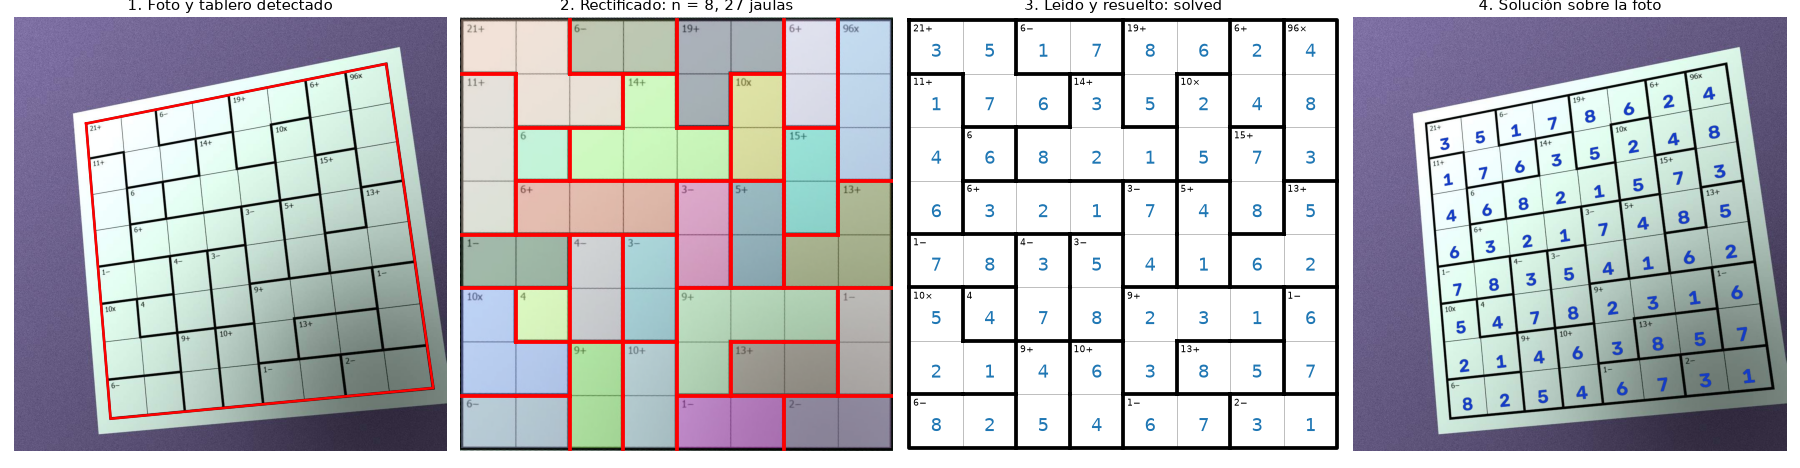
\includegraphics[width=\linewidth]{figs/e2e_photo_8x8.png}
\caption{Demostraci\'on de resoluci\'on End-to-End sobre una fotograf\'{\i}a real de KenKen $8 \times 8$: integraci\'on continua desde la captura inclinada hasta la visualizaci\'on infogr\'afica con superposici\'on de resultados.}
\label{fig:e2e_demo}
\end{figure}

\subsection{Prototipo Interactivo Desplegado en Hugging Face Spaces}
El prototipo fue empaquetado y desplegado p\'ublicamente en la nube en la plataforma \textbf{Hugging Face Spaces} utilizando Gradio, accesible en vivo en \url{https://huggingface.co/spaces/joako2202/kenken-solver}.

La aplicaci\'on integra diagn\'ostico en tiempo real, panel de transparencia con el sem\'aforo de fiabilidad, porcentaje de fidelidad y un cat\'alogo interactivo de 21 muestras operacionales (3 por cada uno de los 7 perfiles).

% ==============================================================================
% SECCIONES FINALES: DISCUSIÓN Y CONCLUSIONES
% ==============================================================================
\section{Discusi\'on y Limitaciones}
\label{sec:discussion}
El cuello de botella sensorial radica en la confusi\'on f\'{\i}sica entre operadores ($\div \leftrightarrow +$). La inferencia conjunta MAP elev\'o la recuperaci\'on exacta del Ground Truth del $4.0\%$ al $58.0\%$ en estr\'es extremo; no obstante, sin regularizaci\'on $\ell_0$ puede derivar en soluciones divergentes. La introducci\'on de la penalizaci\'on $\lambda_{\text{change}} = 1.5$ y la poda sint\'actica a priori resuelven este riesgo de manera determinista.

Como limitaci\'on actual, el sistema asume contornos exteriores rectil\'{\i}neos sobre superficies planas; papel fuertemente doblado o arrugado requerir\'{\i}a t\'ecnicas de desdoblamiento de superficie (\textit{page dewarping}).

\section{Conclusiones}
\label{sec:conclusions}
Se present\'o, formaliz\'o y valid\'o una arquitectura h\'{\i}brida neuro-simb\'olica integral para la resoluci\'on de KenKen:
\begin{enumerate}
    \item La red neuronal \texttt{GlyphCNN} con adaptaci\'on focalizada alcanz\'o una exactitud del $99.51\%$ por glifo y un $90.33\%$ de tableros resueltos en condiciones est\'andar.
    \item El modelado extensional de tabla (Variante B) demostr\'o consistencia GAC, logrando una aceleraci\'on del $39.5\%$ en $n=9$ y resolviendo en nodo ra\'{\i}z con 0 ramas en menos de $13\text{ ms}$.
    \item La regularizaci\'on $\ell_0$ y el sem\'aforo de fiabilidad gradual garantizan un balance \'optimo entre resiliencia sensorial y honestidad algor\'{\i}tmica.
    \item El software opera aut\'onomamente de extremo a extremo y cuenta con un despliegue interactivo accesible en Hugging Face Spaces (\url{https://huggingface.co/spaces/joako2202/kenken-solver}) validado con 90 pruebas unitarias superadas al 100\%.
\end{enumerate}

% ==============================================================================
% REFERENCIAS BIBLIOGRÁFICAS EMBEBIDAS
% ==============================================================================
\begin{thebibliography}{15}

\bibitem{regin1994filtering}
J.-C. R{\'e}gin, ``A filtering algorithm for constraints of difference in CSPs,'' in \emph{AAAI}, vol.~94, pp.~362--367, 1994.

\bibitem{bessiere2006table}
C.~Bessi{\`e}re, E.~Hebrard, B.~Hnich, Z.~Kiziltan, and T.~Walsh, ``Filtering algorithms for table constraints: An overview,'' \emph{Constraints}, vol.~11, no.~4, pp.~271--304, 2006.

\bibitem{ohrimenko2009lazy}
O.~Ohrimenko, P.~J. Stuckey, and M.~Codish, ``Propagation = lazy clause generation,'' in \emph{Principles and Practice of Constraint Programming (CP)}, pp.~444--458, Springer, 2009.

\bibitem{perron2023cpsat}
L.~Perron, F.~Didier, and S.~Gay, ``The {CP-SAT-LP} solver (invited talk),'' in \emph{29th Int. Conf. on Principles and Practice of Constraint Programming (CP 2023)}, vol.~280, pp.~3:1--3:2, Schloss Dagstuhl, 2023.

\bibitem{perron2024ortools}
L.~Perron and V.~Furnon, ``Google {OR-Tools}: Software suite for combinatorial optimization,'' disponible en \url{https://developers.google.com/optimization}, 2024.

\bibitem{deraedt2011constraint}
L.~De~Raedt, T.~Guns, and S.~Nijssen, ``Constraint programming for data mining and machine learning,'' in \emph{Proc. AAAI Conf. on Human Computation and Crowdsourcing}, 2011.

\bibitem{bradski2000opencv}
G.~Bradski, ``The {OpenCV} Library,'' \emph{Dr. Dobb's Journal: Software Tools for the Professional Programmer}, vol.~25, no.~11, pp.~120--123, 2000.

\bibitem{otsu1979threshold}
N.~Otsu, ``A threshold selection method from gray-level histograms,'' \emph{IEEE Trans. Systems, Man, and Cybernetics}, vol.~9, no.~1, pp.~62--66, 1979.

\bibitem{tarjan1975efficiency}
R.~E. Tarjan, ``Efficiency of a good but not linear set union algorithm,'' \emph{Journal of the ACM}, vol.~22, no.~2, pp.~215--225, 1975.

\bibitem{lin2017focal}
T.-Y. Lin, P.~Goyal, R.~Girshick, K.~He, and P.~Doll{\'a}r, ``Focal loss for dense object detection,'' in \emph{Proc. IEEE Int. Conf. on Computer Vision (ICCV)}, pp.~2980--2988, 2017.

\bibitem{chow1970optimum}
C.~Chow, ``On optimum recognition error and reject tradeoff,'' \emph{IEEE Trans. Information Theory}, vol.~16, no.~1, pp.~41--46, 1970.

\bibitem{cortes2016learning}
C.~Cortes, G.~DeSalvo, and M.~Mohri, ``Learning with rejection,'' in \emph{Algorithmic Learning Theory (ALT)}, pp.~67--82, Springer, 2016.

\end{thebibliography}

\end{document}
